\documentclass[12pt,a4paper]{article}

\usepackage{graphicx}% Include figure files
\usepackage{dcolumn}% Align table columns on decimal point
\usepackage{bm}% bold math
%\usepackage{hyperref}% add hypertext capabilities
%\usepackage[mathlines]{lineno}% Enable numbering of text and display math
%\linenumbers\relax % Commence numbering lines

%\usepackage[showframe,%Uncomment any one of the following lines to test 
%%scale=0.7, marginratio={1:1, 2:3}, ignoreall,% default settings
%%text={7in,10in},centering,
%%margin=1.5in,
%%total={6.5in,8.75in}, top=1.2in, left=0.9in, includefoot,
%%height=10in,a5paper,hmargin={3cm,0.8in},
%]{geometry}

\usepackage{multicol}%Para hacer varias columnas
\usepackage{multicol,caption}
\usepackage{multirow}
\usepackage{cancel}
\usepackage{hyperref}
\hypersetup{
    colorlinks=true,
    linkcolor=blue,
    filecolor=magenta,      
    urlcolor=cyan,
}

\setlength{\topmargin}{-1.0in}
\setlength{\oddsidemargin}{-0.3pc}
\setlength{\evensidemargin}{-0.3pc}
\setlength{\textwidth}{6.75in}
\setlength{\textheight}{9.5in}
\setlength{\parskip}{0.5pc}

\usepackage[utf8]{inputenc}
\usepackage{expl3,xparse,xcoffins,titling,kantlipsum}
\usepackage{graphicx}
\usepackage{xcolor} 
\usepackage{nopageno}
\usepackage{lettrine}
\usepackage{caption}
\renewcommand{\figurename}{Figura}
\usepackage{float}
\renewcommand\refname{Bibliograf\'ia}
\usepackage{amssymb}
\usepackage{amsmath}
\usepackage[rightcaption]{sidecap}
\usepackage[spanish]{babel}

\providecommand{\abs}[1]{\lvert#1\rvert}
\providecommand{\norm}[1]{\lVert#1\rVert}
\newcommand{\dbar}{\mathchar'26\mkern-12mu d}

% CABECERA Y PIE DE PÁGINA %%%%%
\usepackage{fancyhdr}
\pagestyle{fancy}
\fancyhf{}

\begin{document}

para el caso no caótico se uso el siguiente código con ángulo inicial 0.2 y 0.201,  aunque variando la subrutina de despliega para poder graficar $\ln{|\theta_1-\theta_2|}$ y $|\theta_1 - \theta_2|$
\begin{verbatim}
    PROGRAM Euler_Cromer
!*********************************************************************
! Se resuelve el pendulo no-lineal, amortiguado y con forzamiento
!
!
!**********************************************************************

 REAL*8, DIMENSION(:), ALLOCATABLE :: theta1,theta2,omega1,omega2,t
 REAL*8 :: length,dt
 INTEGER*8 :: n=15000
!

! print*,"numero de pasos"
! read*, n   ! n=10000
 ALLOCATE (theta1(0:n),theta2(0:n),omega1(0:n),omega2(0:n),t(0:n))
!
!
 call inicializa(theta1, omega1, t, n, length, dt)
 call inicializa(theta2,omega2,t,n,length,dt)
 call calcula(theta1, omega1, t, n, length, dt)
 call calcula(theta2,omega2,t,n,length,dt) 
 call despliega (theta1,theta2,t, n, length, dt)
!
END PROGRAM Euler_Cromer
!
!
SUBROUTINE inicializa(theta, omega, t, n ,length, dt)
 INTEGER*8, INTENT (IN) :: n
 REAL*8, DIMENSION(0:n) :: theta,omega,t
 REAL*8 :: length,dt
 print*,'Angulo inicial del pendulo (en radianes)'
 read*, theta(0)
 !print*,'Velocidad angular inicial del pendulo (en radianes/s)'
 !read*, omega(0)
 omega(0)=0
 t(0)=0.
 !print*,'Longitud del pendulo (in m)'
 !read*, length
 length=9.8d0
! print*, 'Tamaño de paso (en segundos)'
 !read*, dt
 dt = 0.004d0
END SUBROUTINE inicializa
!
!
SUBROUTINE calcula(theta, omega, t, n, length, dt)
 INTEGER*8, INTENT (IN) :: n
 REAL*8, DIMENSION(0:n) :: theta,omega,t
 REAL*8 :: length,dt,g,periodo
 INTEGER :: i
 PI= 4.*ATAN(1.)
 i= 0
 g= 9.80d0
 q=1/2.0d0
 !print*," Amplitud de la fuerza"
 !read*, df
 df=0.5d0
 dfr=2/3.d0
 DO
 omega(i+1) = omega(i) - (g/length) *sin(theta(i)) * dt - q * omega(i)*dt+df*sin(dfr*t(i))*dt
 theta(i+1) = theta(i) + omega(i+1) * dt ! Metodo de Cromer
 if (theta(i+1) > PI ) theta(i+1)=theta(i+1)-2.*PI
 if (theta(i+1) < -PI) theta(i+1)=theta(i+1)+2.*PI
 t(i+1) = t(i) + dt
 IF (i >= n-1) EXIT
 i=i+1
 ENDDO
END SUBROUTINE calcula
SUBROUTINE despliega(theta1,theta2, t, n, length, dt)
 INTEGER*8, INTENT (IN) :: n
 REAL*8, DIMENSION(0:n) :: theta,theta1,theta2,t
 REAL*8 :: length,dt
 INTEGER :: i
 CHARACTER(LEN=10), PARAMETER :: f1 = '(3ES16.6)'
 
 !print*," archivo de datos"
 !read*, archivo
 do i=1, n, 1
  theta(i)= ABS(theta1(i)-theta2(i))
 end do
 OPEN (UNIT=10,FILE="0p5.dat",STATUS='UNKNOWN')
 !
 do i=1 , n ,10
  WRITE(10,f1) theta(i),t(i)
 end do
 !
 CLOSE(10)
END SUBROUTINE despliega
\end{verbatim}

\begin{figure}
    \centering
    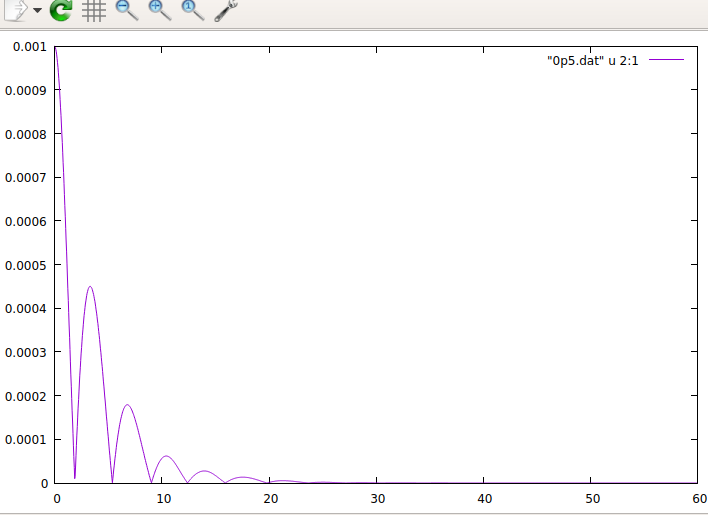
\includegraphics[scale=0.7]{0p5abs.PNG}
    \caption{$|\theta_1-\theta_2|$ vs $t$}
\end{figure}

\begin{figure}
    \centering
    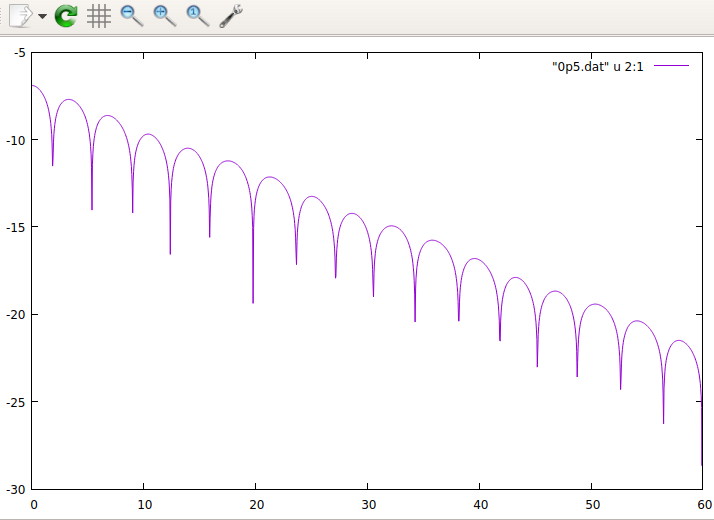
\includegraphics[scale=0.7]{0p5logabs.PNG}
    \caption{$\ln{|\theta_1-\theta_2|}$ vs $t$}
\end{figure}

para el caso caótico se uso el siguiente código con ángulo inicial 0.2 y 0.201,  aunque variando la subrutina de despliega para poder graficar $\ln{|\theta_1-\theta_2|}$ y $|\theta_1 - \theta_2|$

\begin{verbatim}
    PROGRAM Euler_Cromer
!*********************************************************************
! Se resuelve el pendulo no-lineal, amortiguado y con forzamiento
!
!
!**********************************************************************

 REAL*8, DIMENSION(:), ALLOCATABLE :: theta1,theta2,omega1,omega2,t
 REAL*8 :: length,dt
 INTEGER*8 :: n=40000
!

! print*,"numero de pasos"
! read*, n   ! n=10000
 ALLOCATE (theta1(0:n),theta2(0:n),omega1(0:n),omega2(0:n),t(0:n))
!
!
 call inicializa(theta1, omega1, t, n, length, dt)
 call inicializa(theta2,omega2,t,n,length,dt)
 call calcula(theta1, omega1, t, n, length, dt)
 call calcula(theta2,omega2,t,n,length,dt) 
 call despliega (theta1,theta2,t, n, length, dt)
!
END PROGRAM Euler_Cromer
!
!
SUBROUTINE inicializa(theta, omega, t, n ,length, dt)
 INTEGER*8, INTENT (IN) :: n
 REAL*8, DIMENSION(0:n) :: theta,omega,t
 REAL*8 :: length,dt
 print*,'Angulo inicial del pendulo (en radianes)'
 read*, theta(0)
 !print*,'Velocidad angular inicial del pendulo (en radianes/s)'
 !read*, omega(0)
 omega(0)=0
 t(0)=0.
 !print*,'Longitud del pendulo (in m)'
 !read*, length
 length=9.8d0
 !print*, 'Tamaño de paso (en segundos)'
 !read*, dt
 dt=0.004d0
END SUBROUTINE inicializa
!
!
SUBROUTINE calcula(theta, omega, t, n, length, dt)
 INTEGER*8, INTENT (IN) :: n
 REAL*8, DIMENSION(0:n) :: theta,omega,t
 REAL*8 :: length,dt,g,periodo
 INTEGER :: i
 PI= 4.*ATAN(1.)
 i= 0
 g= 9.80d0
 q=1/2.0d0
 !print*," Amplitud de la fuerza"
 !read*, df
 df=1.20d0
 dfr=2/3.d0
 DO
 omega(i+1) = omega(i) - (g/length) *sin(theta(i)) * dt - q * omega(i)*dt+df*sin(dfr*t(i))*dt
 theta(i+1) = theta(i) + omega(i+1) * dt ! Metodo de Cromer
 if (theta(i+1) > PI ) theta(i+1)=theta(i+1)-2.*PI
 if (theta(i+1) < -PI) theta(i+1)=theta(i+1)+2.*PI
 t(i+1) = t(i) + dt
 IF (i >= n-1) EXIT
 i=i+1
 ENDDO
END SUBROUTINE calcula
SUBROUTINE despliega(theta1,theta2, t, n, length, dt)
 INTEGER*8, INTENT (IN) :: n
 REAL*8, DIMENSION(0:n) :: theta,theta1,theta2,t
 REAL*8 :: length,dt
 INTEGER :: i
 CHARACTER(LEN=10), PARAMETER :: f1 = '(3ES16.6)'
 
 !print*," archivo de datos"
 !read*, archivo
 do i=1, n, 1
  theta(i)=LOG(ABS(theta1(i)-theta2(i)))
 end do
 
 OPEN (UNIT=10,FILE="1p2.dat",STATUS='UNKNOWN')
 !
 do i=1, n, 10
  WRITE(10,f1) theta(i),t(i)
 end do
 !
 CLOSE(10)
END SUBROUTINE despliega
\end{verbatim}

\begin{figure}
    \centering
    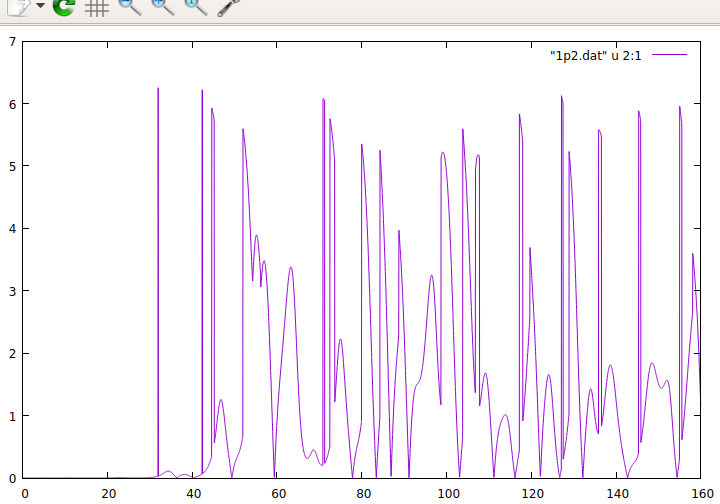
\includegraphics[scale=0.7]{1p2abs.PNG}
    \caption{$|\theta_1-\theta_2|$ vs $t$}
\end{figure}

\begin{figure}
    \centering
    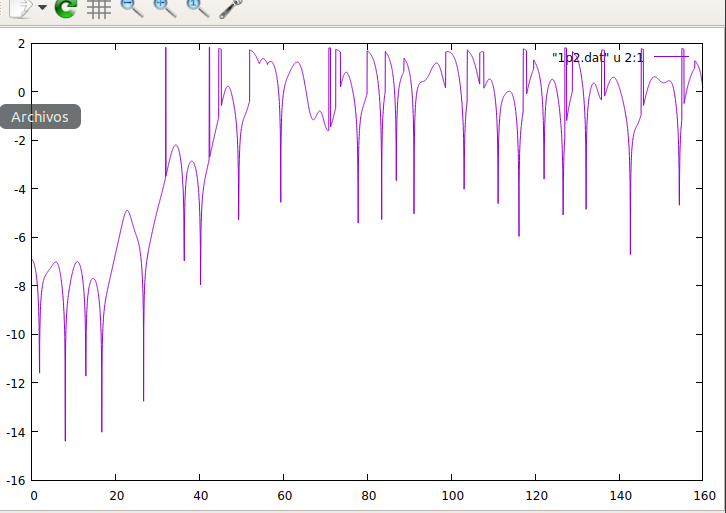
\includegraphics[scale=0.7]{1p2logabs.PNG}
    \caption{$\ln{|\theta_1-\theta_2|}$ vs $t$}
\end{figure}

\end{document}